The final stage of our offline training was estimating a value function $v_p(s)$ that predicts the outcome from position $s$ of games played by using policy $p$ for both players. The goal is to converge to an optimal value function, $v^*(s)$, under perfect play. Silver et al.\cite{b12} estimated the value function $v^{p_\rho}(s)$ for the strongest RL policy network $p_\rho$. The value function was approximated using a value network $v_\theta(s)$ with weights $\theta$, 
% $v_\theta(s) \approx v^{p_\rho}(s) \approx v^*(s)$
\begin{equation}
   v_\theta(s) \approx v^{P_\rho}(s) = E[z_t\ |\ s_t = s, a_{t...T} \sim p] \approx v^*(s).
\end{equation}

This neural network has a similar architecture to the policy network but outputs a single prediction instead of a probability distribution. To train this network, we use the outcomes of the self-play games, $z$, from Sec.~\ref{RL_pn}. From the start to the finish of a game, many board positions from the move sequence can be added to the training dataset, but not more than one board position per game is collected. All board positions in the same game lead to the same result (a win or a loss); they are strongly correlated. To train a model effectively, samples in the training dataset need to be independent. Therefore, we use the RL policy network to play more than 30 million games and collect only one position from each game into the training dataset. We train the weights by regression on these state-outcome pairs $(s, z)$, using stochastic gradient descent to minimize the mean squared error (MSE) between the predicted value $v_\theta(s)$, and the corresponding outcome $z$,
\begin{equation}
    \nabla \theta \propto \frac{\partial v_\theta(s)}{\partial \theta} (z - v_\theta(s)).
\end{equation}
Training on this data set led to MSEs of 0.226 and 0.234 on the training and test set, respectively, indicating minimal overfitting. Fig.~\ref{RL_accu} shows the position evaluation accuracy of the value network, compared to Monte Carlo rollout outcomes using the fast rollout policy $p_\pi$; the value function was consistently more accurate. A single evaluation of $v_\theta(s)$ also approached the accuracy of Monte Carlo rollouts using the RL policy network $p_\rho$ but using 15,000 times less computation.

\begin{figure}[t]
\centerline{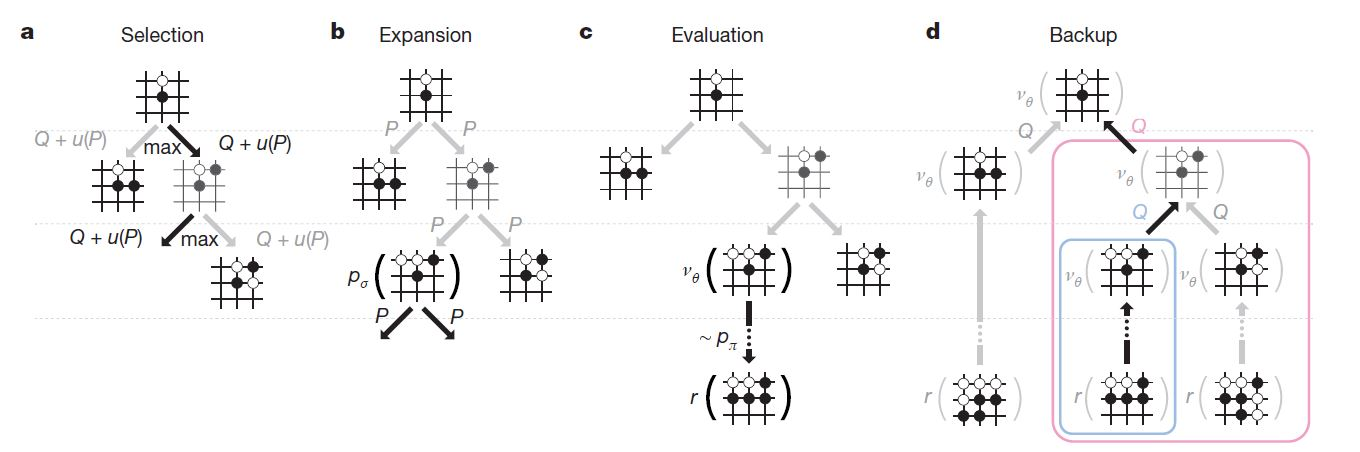
\includegraphics[width = \columnwidth]{MCTS.JPG}}
\caption{Monte Carlo tree-search in AlphaGO\cite{b12}}
\label{MCTS_1}
\end{figure}